\documentclass[11pt,oneside]{article}
\usepackage[T1]{fontenc}
\usepackage[utf8]{inputenc}
%\DeclareUnicodeCharacter{00A0}{ }
\usepackage[adobe-utopia]{mathdesign}

\usepackage{amsmath}
\usepackage[francais]{babel}
\usepackage[dvips]{graphicx}
%\usepackage{here}
\usepackage{framed}
\usepackage[normalem]{ulem}
\usepackage{fancyhdr}
\usepackage{titlesec}
\usepackage{vmargin}

\usepackage{amsmath}
\usepackage{ifthen}
\usepackage{multirow}
\usepackage{multicol} % Portions de texte en colonnes

%\usepackage{xltxtra} % Logo XeLaTeX
%\usepackage{pst-solides3d}
\usepackage{color}
%\usepackage{colortbl}
\usepackage{titletoc} % Pour la mise en forme de la table des matières

%\usepackage[crop=off]{auto-pst-pdf}
%\usepackage{bclogo}


%\usepackage{longtable}
%\usepackage{flafter}%floatants après la référence
%\usepackage{pst-solides3d}
%\usepackage{pstricks}
%\usepackage{minitoc}
%\setcounter{minitocdepth}{4}
%\usepackage{draftcopy}% "Brouillon"
%\usepackage{floatflt}
%\usepackage{psfrag}
%\usepackage{listings} % Permet d'insérer du code de programmation
%\usepackage{lmodern}
%\usepackage[adobe-utopia,uppercase=upright,greeklowercase=upright]{mathdesign}
%\usepackage{minionpro}
%\usepackage{pifont}
%\usepackage{amssymb}
%\usepackage[francais]{varioref}

\setmarginsrb{1.5cm}{1cm}{1cm}{1.5cm}{1cm}{1cm}{1cm}{1cm}

\definecolor{gris25}{gray}{0.75}
\definecolor{bleu}{RGB}{18,33,98}
\definecolor{bleuf}{RGB}{42,94,171}
\definecolor{bleuc}{RGB}{231,239,247}
\definecolor{rougef}{RGB}{185,18,27}
\definecolor{rougec}{RGB}{255,230,231}
\definecolor{vertf}{RGB}{103,126,82}
\definecolor{vertc}{RGB}{220,255,191}
\definecolor{violetf}{RGB}{112,48,160}
\definecolor{violetc}{RGB}{230,224,236}
\definecolor{jaunec}{RGB}{220,255,191}
\usepackage[raccourcis]{FAST}
\usepackage[%
    pdftitle={Conception -- Liaisons encastrement},
    pdfauthor={Xavier Pessoles},
    colorlinks=true,
    linkcolor=blue,
    citecolor=magenta]{hyperref}
\usepackage{schemabloc}



% \makeatletter \let\ps@plain\ps@empty \makeatother
%% DEBUT DU DOCUMENT
%% =================
\sloppy
\hyphenpenalty 10000

\newcommand{\Pointilles}[1][3]{%
\multido{}{#1}{\makebox[\linewidth]{\dotfill}\\[\parskip]
}}


\colorlet{shadecolor}{orange!15}

\newtheorem{theorem}{Theorem}


\begin{document}


\newboolean{prof}
\setboolean{prof}{true}
%------------- En tetes et Pieds de Pages ------------
\pagestyle{fancy}
\renewcommand{\headrulewidth}{0pt}

\fancyhead{}
\fancyhead[L]{%
\noindent\noindent\begin{minipage}[c]{2.6cm}
%Lycée Rouvière PTSI

\includegraphics[width=2cm]{png/logo_ptsi.png}%
\end{minipage}
}

\fancyhead[C]{\rule{12cm}{.5pt}}

\fancyhead[R]{%
\noindent\begin{minipage}[c]{3cm}
\begin{flushright}
\footnotesize{\textit{\textsf{Sciences Industrielles\\ pour l'Ingénieur}}}%
\end{flushright}
\end{minipage}
}

\renewcommand{\footrulewidth}{0.2pt}

\fancyfoot[C]{\footnotesize{\bfseries \thepage}}
\fancyfoot[L]{\footnotesize{2012 -- 2013} \\ X. \textsc{Pessoles}}
\ifthenelse{\boolean{prof}}{%
\fancyfoot[R]{\footnotesize{Cours -- CI : Conception -- P}}
}{%
\fancyfoot[R]{\footnotesize{Cours -- CI : Conception}}
}



\begin{center}
 \huge\textsc{CI 4 -- Conception : Conception des mécanismes}
\end{center}

\begin{center}
 \LARGE\textsc{Chapitre 1 -- Représentation des éléments filetés}
\end{center}

\vspace{.5cm}

\begin{center}
\begin{tabular}{ccc}
%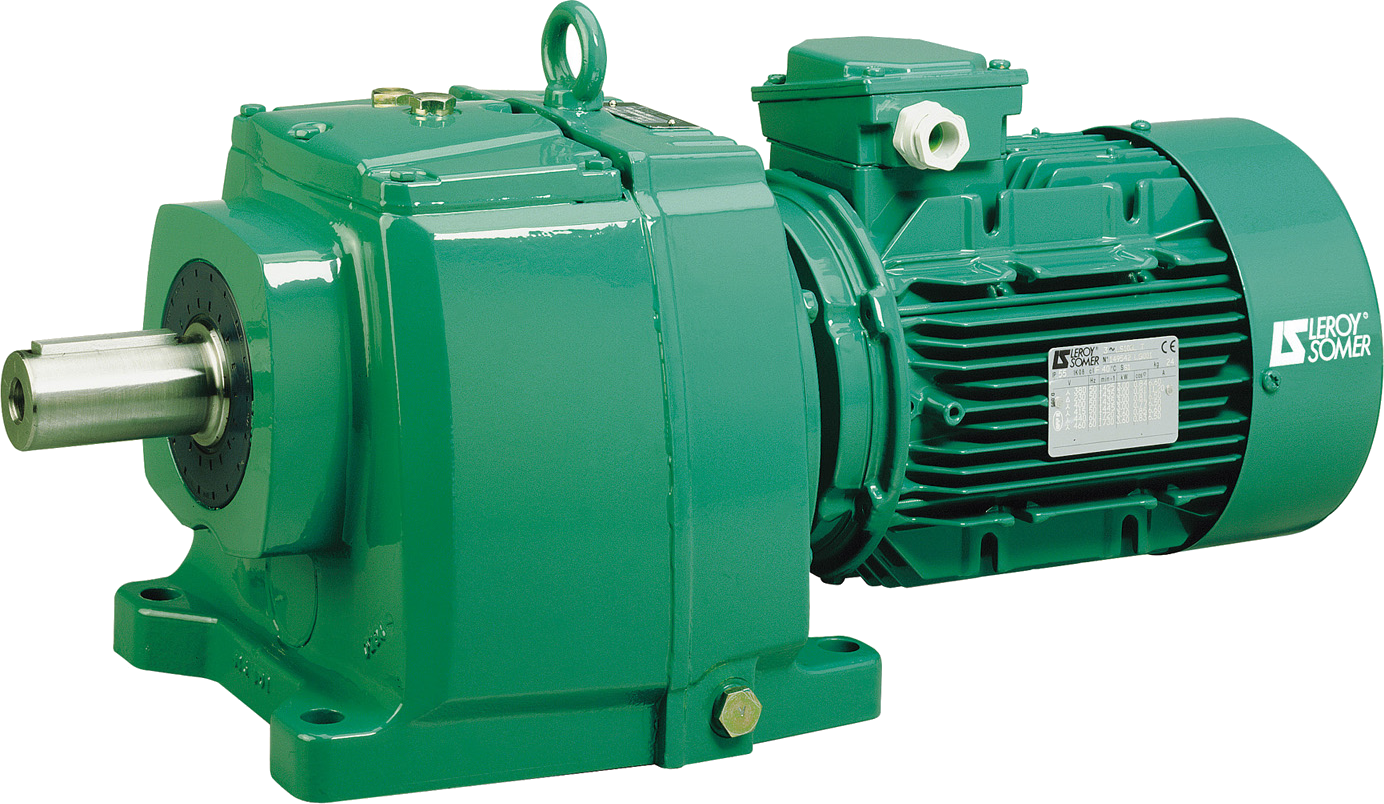
\includegraphics[height=3cm]{png/motored1} &
%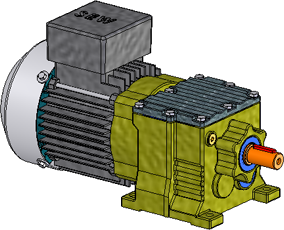
\includegraphics[height=3cm]{png/motored2} &
%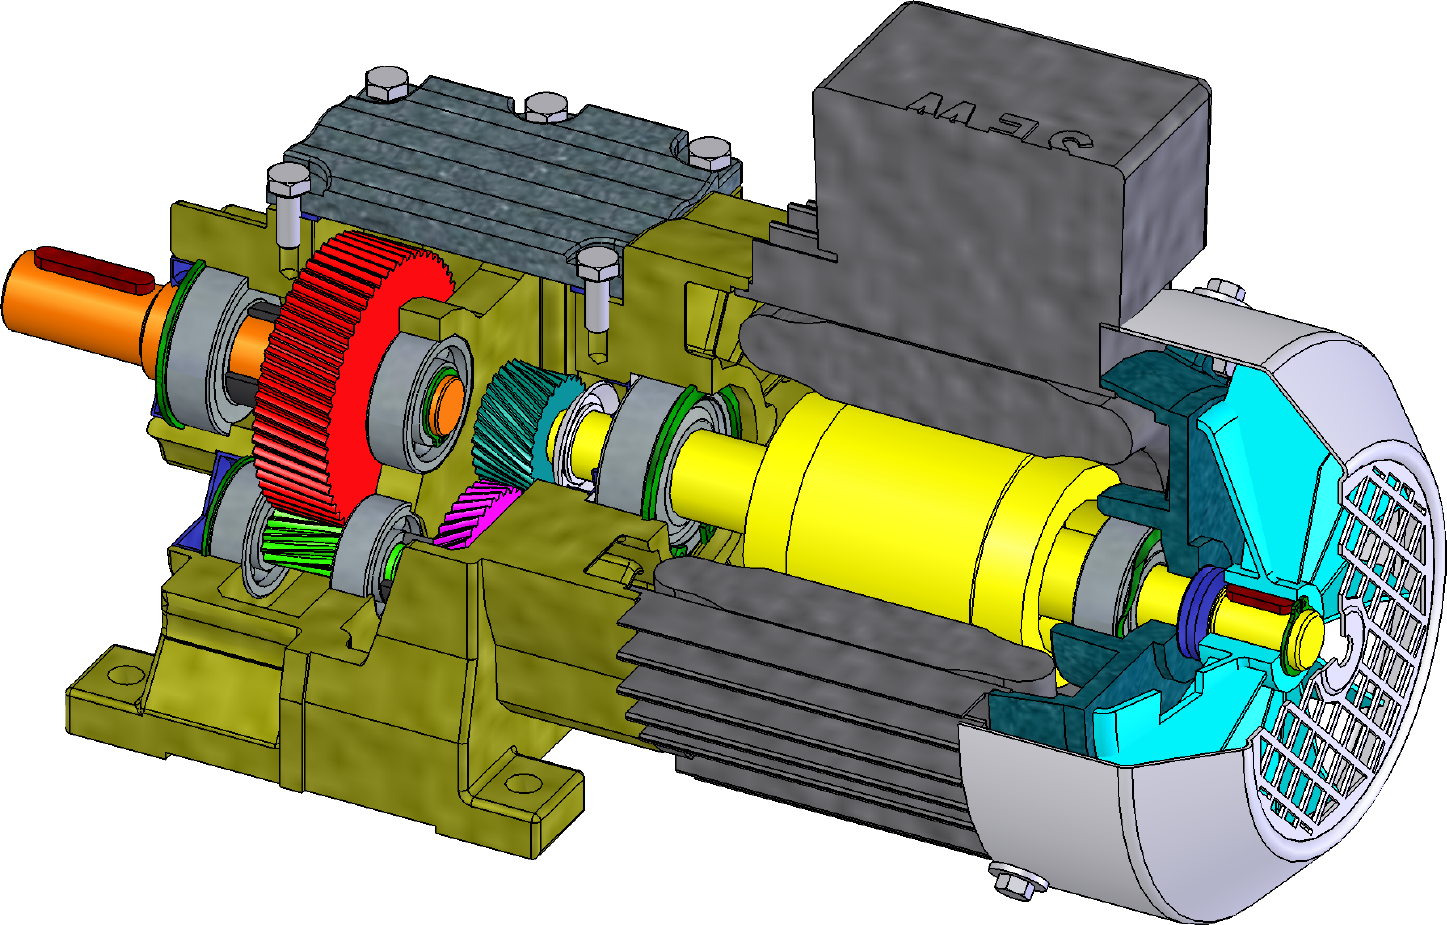
\includegraphics[height=3cm]{png/motored3} \\
%\textit{Motoréducteur Leroy Somer \cite{ls}} & \textit{Motoréducteur SEW}&\textit{Écorché}\\
\end{tabular}
\end{center}

Les éléments filetés sont au c\oe{}ur de la conception des systèmes mécaniques. Ils constituent une solution technologique pour assembler des pièces les unes avec les autres. 

Il est dans un premier temps nécessaire de reconnaître les assemblages filetés dans les mécanismes afin de repérer les classes d'équivalences. Dans un second temps, il est nécessaire de savoir les représenter dans le but de concevoir des systèmes robustes.

Les liaisons assurées par des éléments filetés sont pour la plupart démontables afin de pouvoir effectuer la maintenance du système. Elles jouent un rôle clé dans la conception des liaisons encastrement démontables. Ces dernières seront utilisées ultérieurement.




\begin{prob}
\textsc{Problématique :}
\begin{itemize}
\item Utiliser un assemblage fileté quand les conditions de fonctionnement l'imposent
\end{itemize}
\end{prob}

\begin{savoir}
\textsc{Savoirs :}
\begin{itemize}
\item Représenter un assemblage fileté
\end{itemize}
\end{savoir}

%\newpage 

\setlength{\parskip}{0ex plus 0.2ex minus 0ex}
 \renewcommand{\contentsname}{}
 \renewcommand{\baselinestretch}{1}

\tableofcontents

 \renewcommand{\baselinestretch}{1.2}
\setlength{\parskip}{2ex plus 0.5ex minus 0.2ex}

% \vspace{1cm}
\textit{Ce document est en évolution permanente. Merci de signaler toutes
erreurs ou coquilles.}

%\newpage



\section{Éléments filetés et taraudés}
Les éléments filetés et taraudés regroupent les vis, les écrous, mais aussi les pièces fabriquées par tournage ou fraisage présentant un filet hélicoïdal. Bien qu'il existe des profils de vis trapézoïdaux ou ronds, le profil le plus utilisé est le \textbf{profil métrique ISO} (profil triangulaire).

\subsection{Représentation des filetages et des taraudages}
\subsubsection{Trou taraudé débouchant}

\begin{center}
\includegraphics[width=.6\textwidth]{png/taraudage_debouchant_e}
\end{center}

\subsubsection{Trou taraudé borgne}

\begin{center}
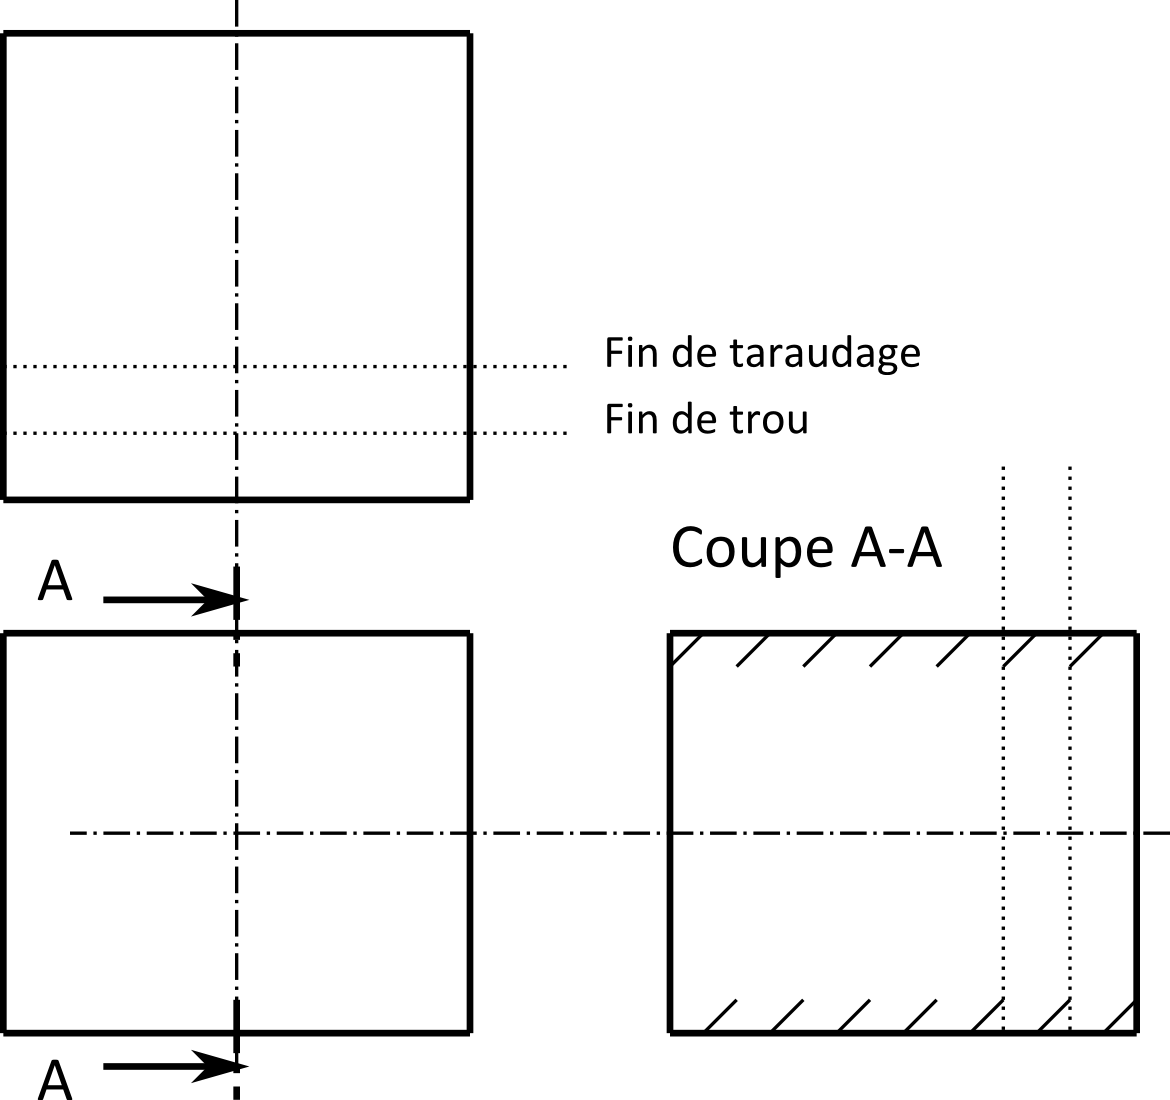
\includegraphics[width=.6\textwidth]{png/taraudage_borgne_e}
\end{center}

\subsubsection{Vis d'assemblage}
\begin{defi}

Tige filetée munie d'une tête permettant l'entrainement en rotation. La vis traverse la pièce à serrer par un trou lisse avec jeu. Le serrage provoque la disparition de tout jeu suivant l'axe de la vis. 

\end{defi}

\begin{center}
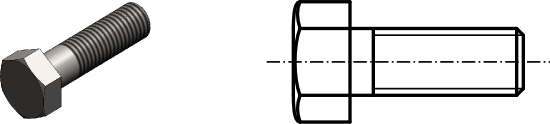
\includegraphics[width=.5\textwidth]{png/vis_rep}
\end{center}

\subsubsection{Tige filetée dans un trou taraudé}
\begin{center}
\includegraphics[width=.8\textwidth]{png/tige_trou}
\end{center}

\subsubsection{Serrage par vis dans trou taraudé}
\begin{center}
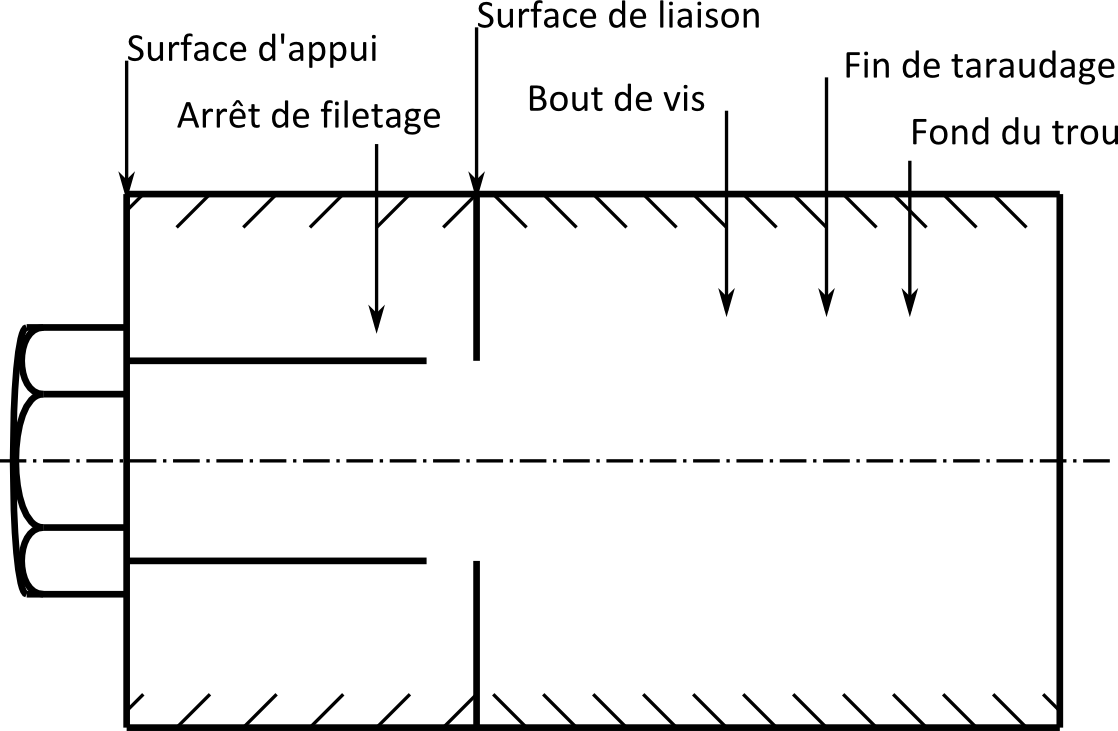
\includegraphics[width=.5\textwidth]{png/serrage_vis}
\end{center}

%\subsubsection{Récapitulatif}
\subsection{Désignation et représentation des vis}


Dans les nomenclatures, les vis sont désignées comme suit : 

\noindent\noindent\begin{minipage}[c]{.46\linewidth}
\begin{center}
NF ISO 4762 -- M10 x 30 -- 8.8
\end{center}
\end{minipage}\hfill
\noindent\begin{minipage}[c]{.46\linewidth}
\begin{itemize}
\item NF ISO 4762 : tête cylindrique à 6 pans creux
\item M : profil ISO (triangulaire)
\item 10 : diamètre nominal de la vis 
\item 30 : longueur filetée (en $mm$)
\item 8.8 : qualité de la vis ($8\times 100=800\; MPa$ : résistance maximale à la traction; $8\times 8 \time 10 = 640 \; MPa$ : limite minimale d'élasticité)
\end{itemize}
\end{minipage}

\vspace{.25cm}
Pour les filets ISO, le pas est directement donné en fonction du diamètre nominal (existence d'un pas gros (le plus courant) ou d'un pas fin).

\subsection{Types de vis et formes de têtes}
Une multitude de type de vis existent en fonction des besoins (vis d'assemblage, vis de pression) et des encombrements disponibles.

En règle générale, les vis hexagonales et les vis cylindriques à embout hexagonal creux restent les plus utilisées. Ces dernières ont la possibilité de voir leurs têtes logées dans des lamages.
\begin{center}
\begin{tabular}{|m{7cm}|m{2.5cm}|m{2cm}|m{2.5cm}|m{2.5cm}|}
\hline
\textbf{Géométrie de la vis} & \textbf{Forme sous tête}  & \textbf{Forme tête} & & \textbf{Remarque}\\
\hline \hline
&&&& \\
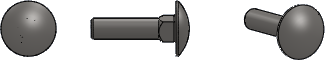
\includegraphics[width=6.5cm]{png/vis_1} &  & \textbf{B} -- Bombée & & Col carré\\
\hline
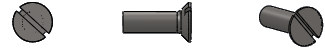
\includegraphics[width=6.5cm]{png/vis_2} &  \textbf{F} -- Fraisée &  & \textbf{S} -- Fendue& \\
\hline
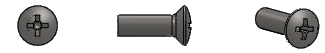
\includegraphics[width=6.5cm]{png/vis_3} & \textbf{F} -- Fraisée & \textbf{B} -- Bombée & \textbf{H} -- Cruciforme& \\
\hline
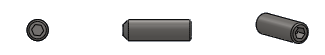
\includegraphics[width=6.5cm]{png/vis_4} & & & \textbf{HC} - hexagonal creux & Vis de pression\\
\hline
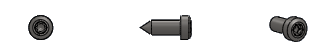
\includegraphics[width=6.5cm]{png/vis_5} & \textbf{C} -- Cylindrique & \textbf{B} - bombée & Torx & Auto foreuse \\
\hline
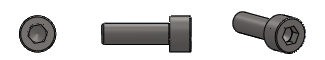
\includegraphics[width=6.5cm]{png/vis_6} & \textbf{C} -- Cylindrique & & \textbf{HC} -- hexagonal creux & \\
\hline
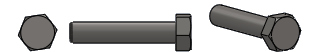
\includegraphics[width=6.5cm]{png/vis_7} & \textbf{H} -- Hexagonale & & & \\
\hline
\end{tabular}
\end{center}




\subsection{Écrous}
\begin{center}
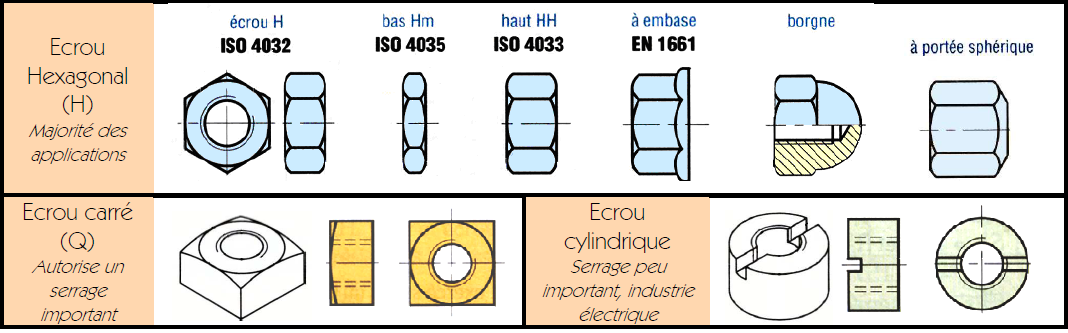
\includegraphics[width=.8\textwidth]{png/ecrous}
\end{center}

%\begin{center}
%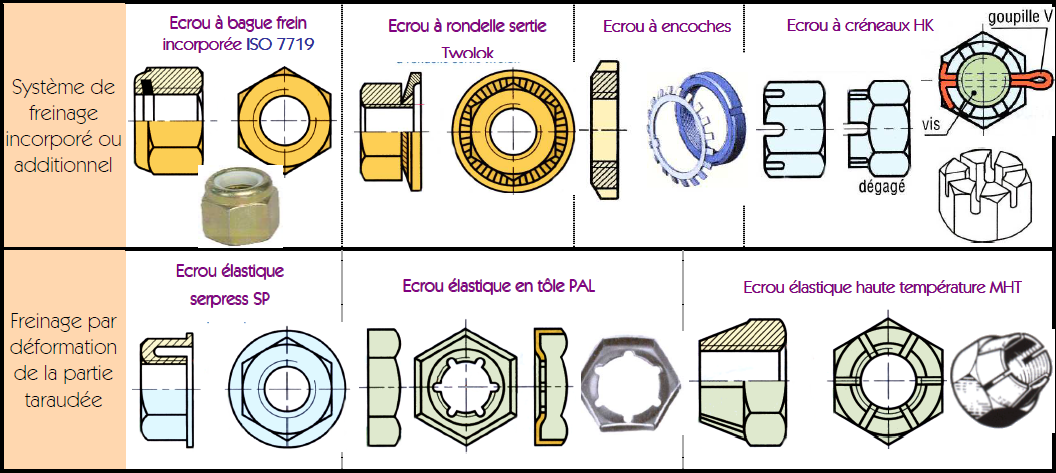
\includegraphics[width=.8\textwidth]{png/ecrous_2}
%\end{center}

%\begin{center}
%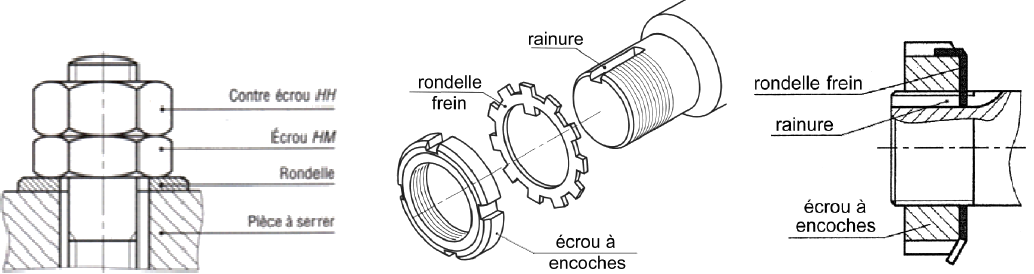
\includegraphics[width=.8\textwidth]{png/ecrous_3}
%\end{center}

\begin{center}
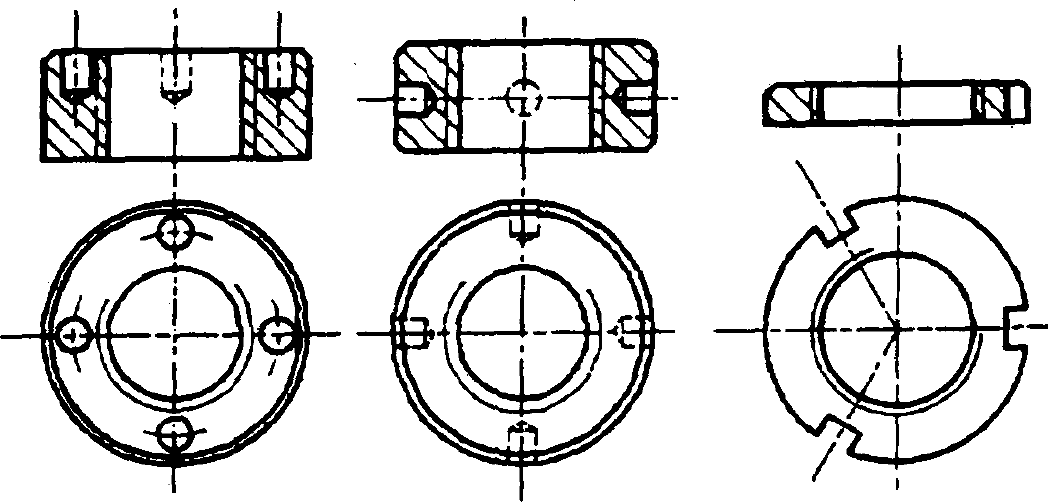
\includegraphics[width=.7\textwidth]{png/ecrous_p}
\end{center}




\subsection{Boulons}
\begin{defi}
\begin{minipage}[c]{.7\linewidth}
Un assemblage boulonné est constitué d'une vis, d'un écrou et des pièces à serrer. Ces dernières sont traversées par un trou lisse avec jeu. Le jeu suivant l'axe de la vis disparaît lors du serrage. 
\end{minipage} \hfill
\begin{minipage}[c]{.25\linewidth}
\begin{center}
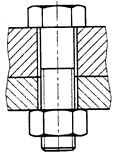
\includegraphics[width=.8\textwidth]{png/boulon}
\end{center}
\end{minipage}
\end{defi}
\subsection{Goujons}

Un goujon est une tige cylindrique filetée aux deux extrémités. Il est vissé à fond de filetage dans une des pièces à assembler à l’aide d’une goujonneuse.
Les goujons sont souvent utilisés pour assembler des pièces ne pouvant être traversées par des vis.
Ils sont également employés dans le cas de pièces en alliage léger, où le démontage trop fréquent de la vis risque de provoquer la détérioration des filets du trou taraudé.


\begin{center}
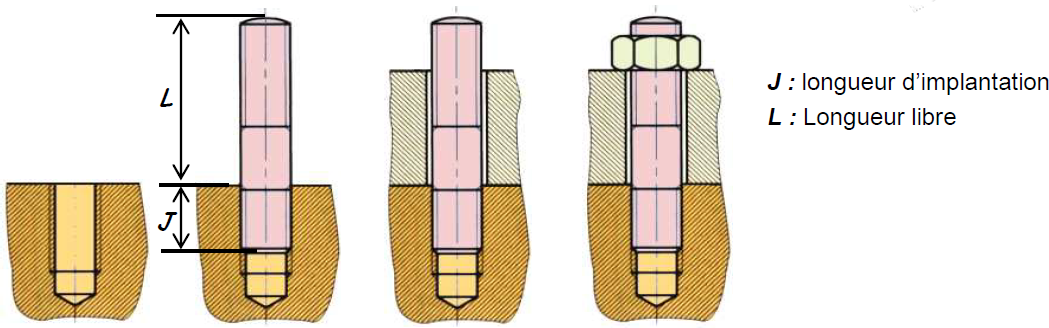
\includegraphics[width=.8\textwidth]{png/goujon}
\end{center}

Pour une vis l’implantation minimale J doit être au moins égale :
\begin{itemize}
\item $J \geq d$, diamètre nominal dans l’acier;
\item $J \geq 1,5 \times d$, diamètre nominal dans la fonte, le cuivre;
\item $J \geq 2 \times d$, diamètre nominal dans l’aluminium.
\end{itemize}
Pour un goujon l'implantation minimale J doit être au moins égale :	 
\begin{itemize}
\item $J \geq 1,5 \times d$, diamètre nominal dans l’acier;
\item $J \geq 2 \times d$, diamètre nominal dans un métal tendre.
\end{itemize}


\subsection{Technologie des éléments filetés}
\paragraph*{Matériaux}
\begin{center}
\begin{tabular}{|c|c|c|c|c|}
\multicolumn{5}{c}{\textbf{Matériaux des vis}} \\ \hline
Catégorie & Matière & État & $\quad Rm \; (MPa) \quad $ & $\quad Re  \; (MPa) \quad $ \\ \hline
Acier non traité & $S\; 235$ & -- & 340 & 235 \\ \hline
Acier traité & $25\;Cr\;Mo\; 4$ & Trempé revenu & 930 & 785 \\ \hline
Acier inoxydable & $X\; 30 \;Cr\;Ni\; 18-10$ & Trempé revenu & 900 & 750 \\ \hline
\end{tabular}
\end{center}

\paragraph*{Fabrication}
Le processus de fabrication des vis est généralement proche de cela : 
\begin{itemize}
\item laminage : obtention de rouleau de fil (le diamètre du fil pouvant aller jusqu'à plusieurs dizaines de $mm$);
\item redressage afin de redresser le rouleau en tige;
\item découpage des tronçons;
\item forgeage à froid (avec plusieurs matrices) de la tête de vis;
\item chanfreinage du bout de vis;
\item roulage du filetage;
\item traitement thermique.
\end{itemize}


Lorsqu'il s'agit de fabriquer des arbres filetés ou des moyeux taraudés, il est possible d'utiliser des procédés de filetage (tournage) ou de taraudage (tournage ou fraisage). 

En tournage, lorsqu'un outil à fileter est utilisé, une gorge doit être réalisée avant un épaulement. Cette dernière empêche ainsi l'outil de de butter contre un plan. 

Lors de l'utilisation d'un taraud sur un centre d'usinage, la broche se doit d'être asservie. En effet, une mauvaise synchronisation des axes provoquerait une casse du filet. 

\noindent\begin{minipage}[c]{.3\linewidth}
\begin{center}
\includegraphics[width=.8\textwidth]{png/taraudage_lisse}
\end{center}

\noindent\textit{Taraudage dans un trou borgne : le trou de perçage réaliser grâce à un foret est plus profond que la partie taraudée.}
\end{minipage}\hfill
\begin{minipage}[c]{.3\linewidth}
\begin{center}
\includegraphics[width=.8\textwidth]{png/taraudage_epaul}
\end{center}

\noindent\textit{Taraudage terminant par un épaulement : ou bien le taraudage s'arrête bien avant l'épaulement, ou bien on prévoit une gorge de dégagement.}
\end{minipage}\hfill
\begin{minipage}[c]{.3\linewidth}
\begin{center}
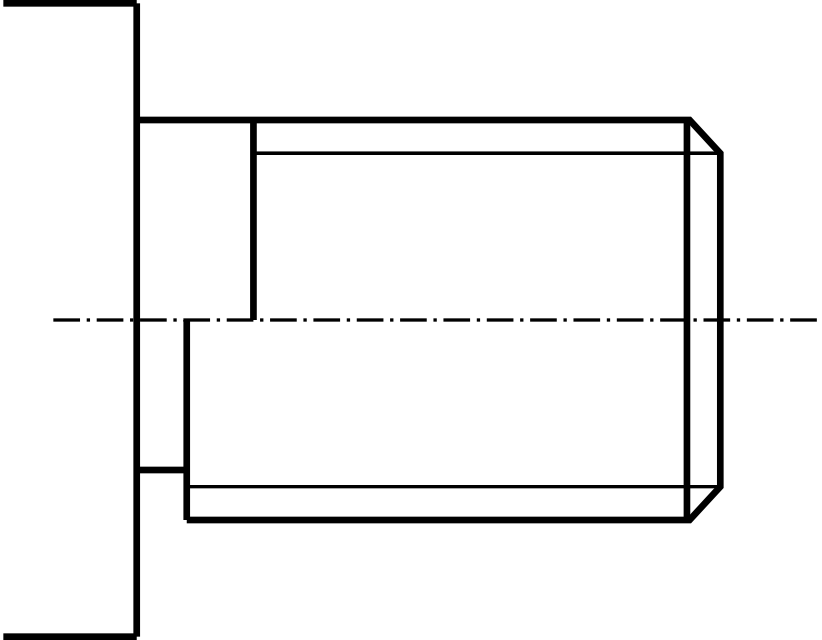
\includegraphics[width=.8\textwidth]{png/epaulement}
\end{center}

\noindent\textit{Filetage terminant par un épaulement : préférer la solution avec une gorge en fin de filetage.}
\end{minipage}


\paragraph*{Classe de qualité}
La classe de qualité de vis est généralement marquée sur la tête. Elle indique le comportement de la vis lorsqu'elle est soumise à des efforts axiaux. Elle est composée de deux chiffres séparés par un point : $a.b$.

$a\times 100$ donne la limite à la rupture de la vis.

$a\times b\times 10$ donne la limite à l'élasticité de la vis. 

Ces valeurs sont déterminées par des essais de traction. 

\textbf{Attention à ne pas solliciter les vis en cisaillement. Il ne faut donc pas utiliser les vis pour assurer une mise en position.}

\begin{center}
\begin{tabular}{|l|c|c|c|c|c|c|c|c|c|c|}
\hline
Classe de résistance & 
$3.6$ & $4.6$ & $4.8$ & $5.6$ & $5.8$ & $6.8$ & $8.8$ & $9.8$ & $10.9$ & $12.9$ \\
\hline 
Limite élastique ($MPa$) & 180 & 240 & 320 & 300 & 400 & 480 & 640 & 720 & 900 & 1 080 \\
\hline
Limite à la rupture  ($MPa$) & 330 & 400 & 420 & 500 & 520 & 600 & 800 & 900 & 1 040 & 1 220 \\
\hline
\end{tabular}
\end{center}

%\subsection{Dimensionnement des assemblages filetés}
%
\section{Réaliser le maintien en position entre pièces}
\subsection{Conception des assemblages vissés}
Maintien en position lors de la mise en position par appui plan prépondérant et centrage court :

\begin{center}
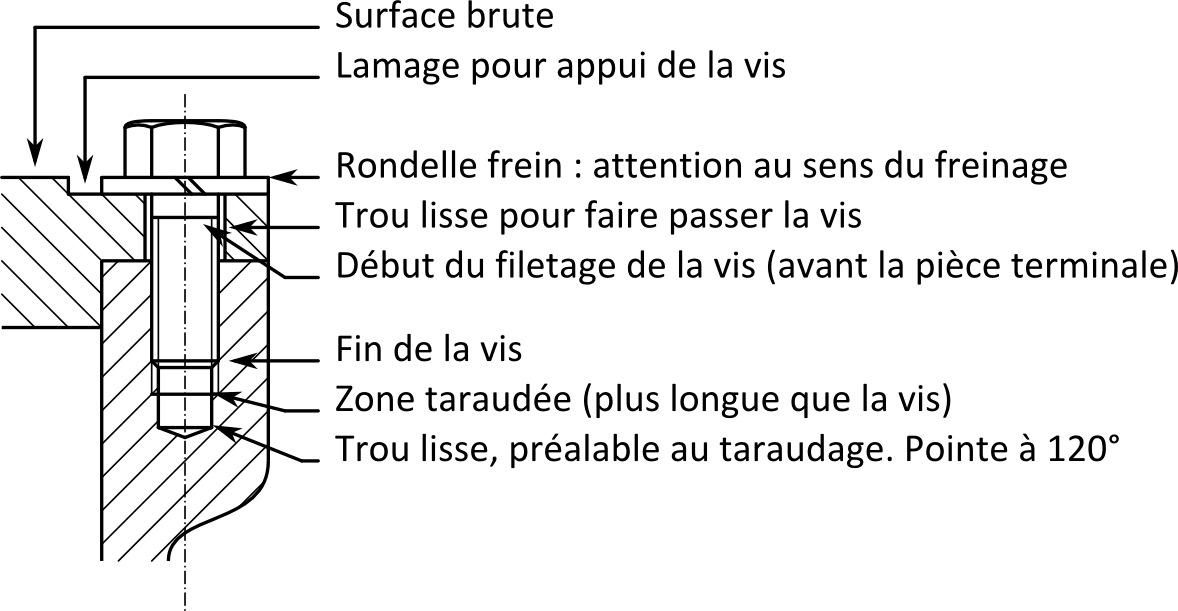
\includegraphics[width=.8\textwidth]{png/Fig30_1}
\end{center}

\noindent\begin{minipage}[c]{.3\linewidth}
\begin{center}
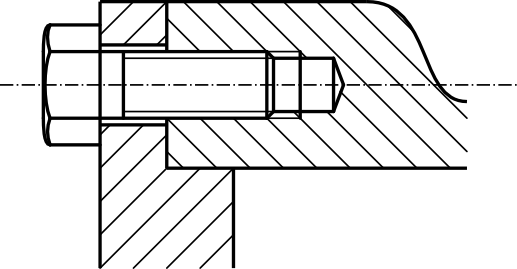
\includegraphics[width=.9\textwidth]{png/Fig30_2}

\textbf{Assemblage avec vis Hexagonale}
\end{center}
\end{minipage}\hfill
\begin{minipage}[c]{.3\linewidth}
\begin{center}
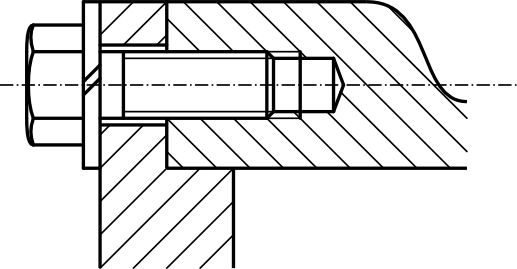
\includegraphics[width=.9\textwidth]{png/Fig30_3}

\textbf{Assemblage avec vis Hexagonale et rondelle frein}
\end{center}
\end{minipage}\hfill
\begin{minipage}[c]{.3\linewidth}
\begin{center}
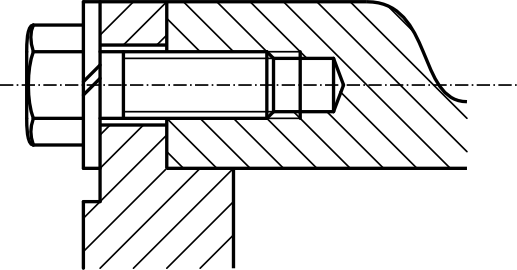
\includegraphics[width=.9\textwidth]{png/Fig30_6}

\textbf{Assemblage avec vis Hexagonale, rondelle frein et lamage}
\end{center}
\end{minipage}

\vspace{.5cm}

\noindent\hspace{.15\textwidth}\begin{minipage}[c]{.3\linewidth}
\begin{center}
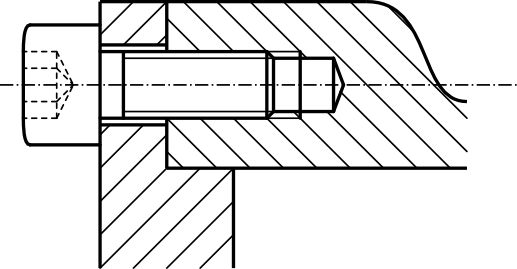
\includegraphics[width=.9\textwidth]{png/Fig30_4}

\textbf{Assemblage avec vis CHC}
\end{center}
\end{minipage}\hfill
\begin{minipage}[c]{.3\linewidth}
\begin{center}
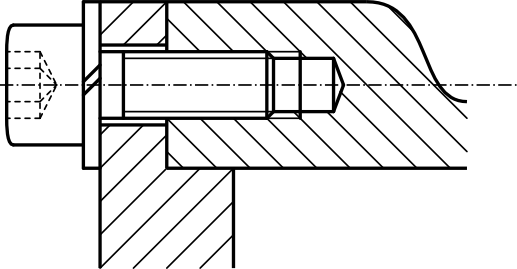
\includegraphics[width=.9\textwidth]{png/Fig30_5}

\textbf{Assemblage avec vis CHC et rondelle frein}
\end{center}
\end{minipage}\hspace{.15\textwidth}


\vspace{.5cm}

Maintien en position lors de la mise en position par centrage long et appui ponctuel :
\begin{center}
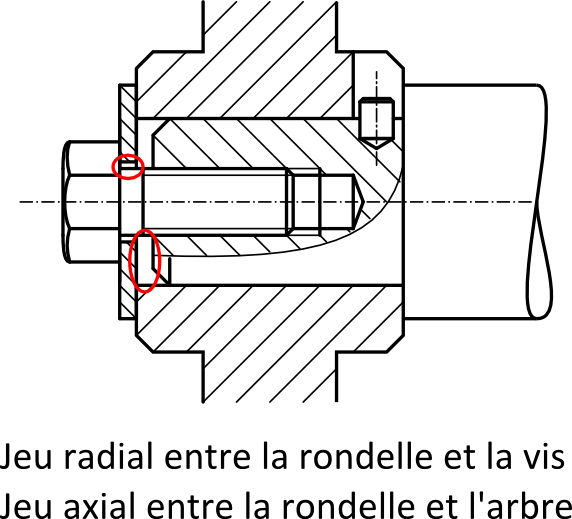
\includegraphics[width=.4\textwidth]{png/Fig31}

\end{center}

\vspace{.5cm}

Suivant la tête de vis utilisée et suivant la provenance du brut, il est possible de donner des formes différentes à la zone de contact entre la tête de vis et le support. 

\begin{center}
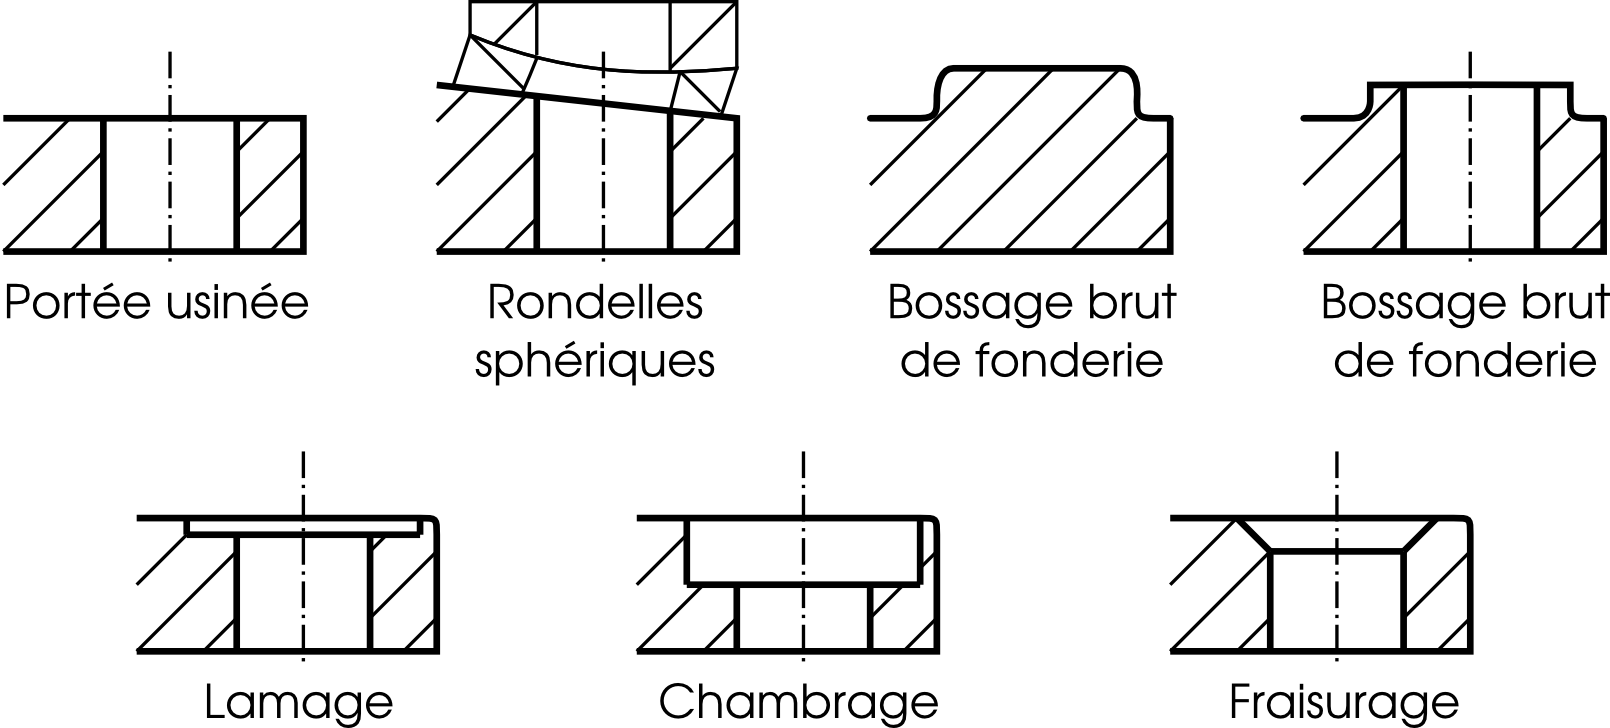
\includegraphics[width=.7\textwidth]{png/portees}
\end{center}



\subsection{Conception des assemblages boulonnés}

On parle d'assemblage boulonné lorsque au moins deux pièces sont maintenues en position par \textbf{une vis et un écrou}. Dans ce cas, les perçages des pièces sont \textbf{lisses}.

\begin{center}
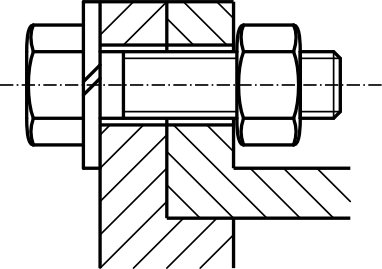
\includegraphics[width=.3\textwidth]{png/Fig30_7}

\end{center}





\section{Assurer l'étanchéité}
Plusieurs solutions permettent d'assurer l'étanchéité d'un mécanisme. Nous nous intéressons ici aux solutions d'étanchéité statique (par "opposition" aux solutions d'étanchéité dynamique).

\noindent\begin{minipage}[c]{.3\linewidth}
\begin{center}
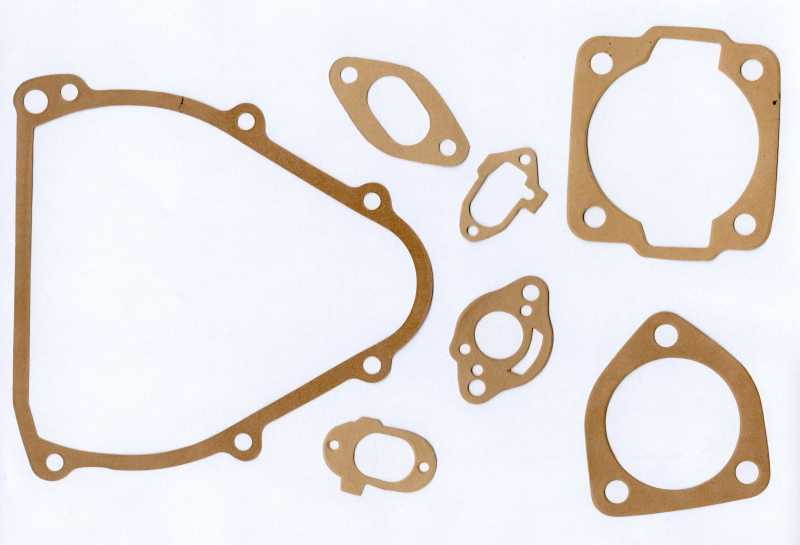
\includegraphics[width=.9\textwidth]{png/papier}

\textit{Joint papier \cite{papier}}
\end{center}
\end{minipage}\hfill
\begin{minipage}[c]{.3\linewidth}
\begin{center}
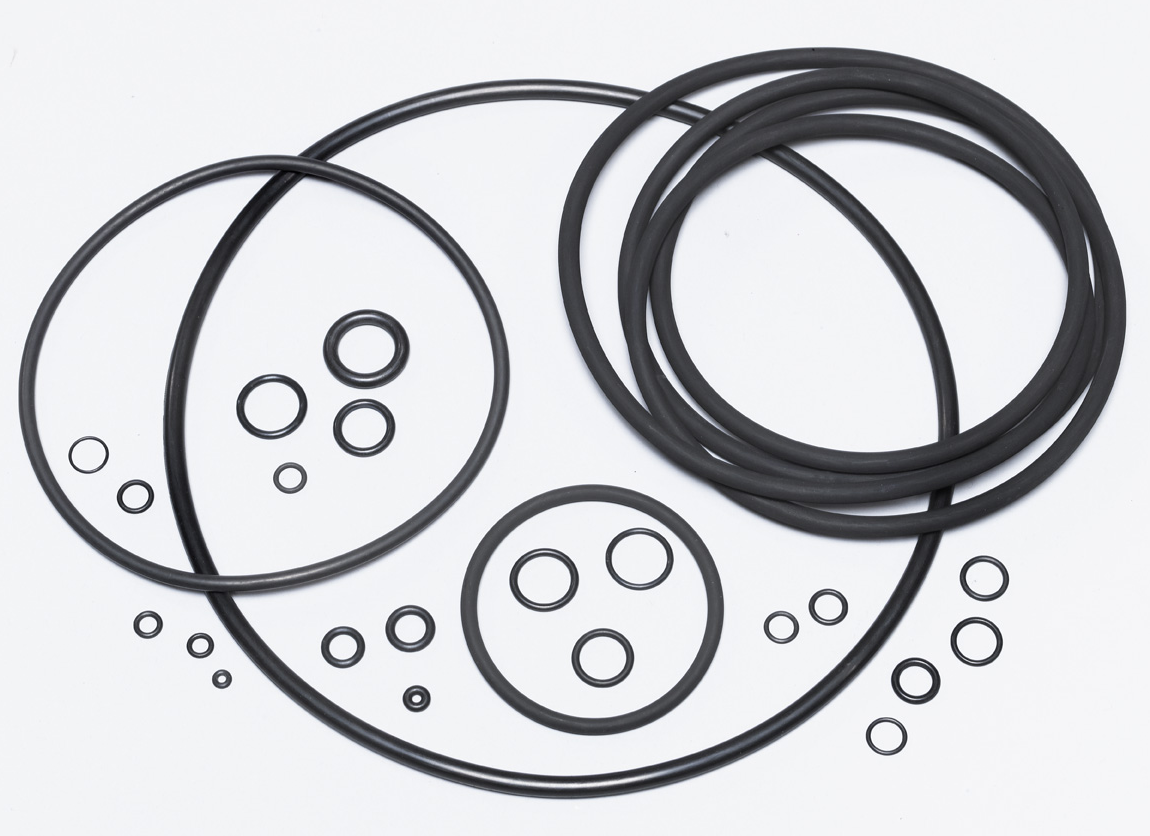
\includegraphics[width=.9\textwidth]{png/torique}

\textit{Joints toriques \cite{torique}}
\end{center}
\end{minipage}\hfill
\begin{minipage}[c]{.3\linewidth}
\begin{center}
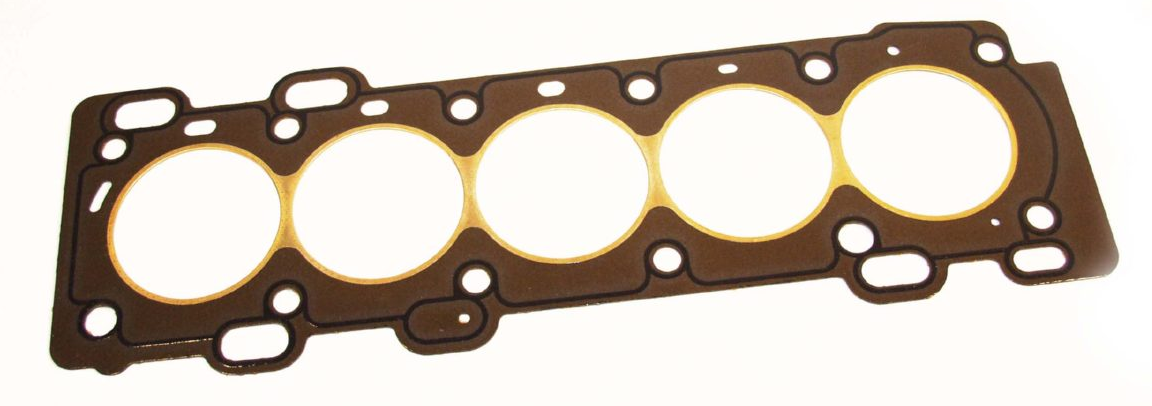
\includegraphics[width=.9\textwidth]{png/culasse}

\textit{Joint de culasse \cite{culasse}}
\end{center}
\end{minipage}


\section{Assurer la fiabilité}
Les chocs, les vibrations répétées, les variations de température auxquels sont soumis les assemblages par
éléments filetés, peuvent très rapidement entraîner leur desserrage (perte de la pression de contact entre
filets de la vis et de l'écrou).


\subsection{Écrous freinés}
\begin{center}
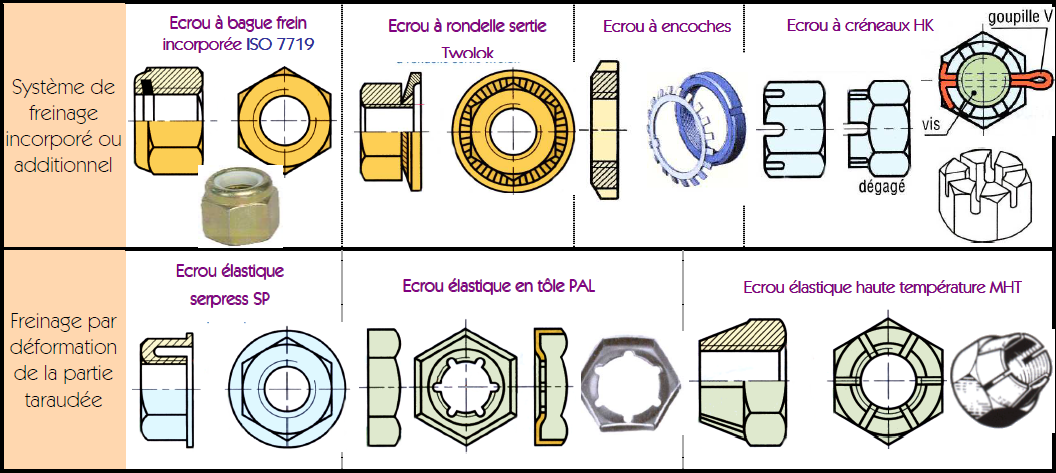
\includegraphics[width=.8\textwidth]{png/ecrous_2}
\end{center}

\begin{center}
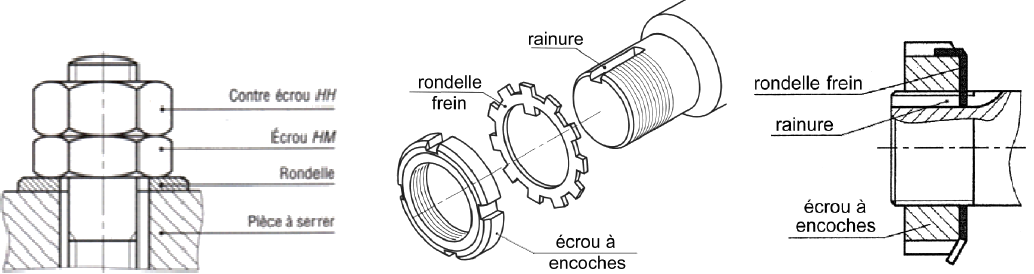
\includegraphics[width=.8\textwidth]{png/ecrous_3}
\end{center}

\subsection{Rondelles}

\begin{center}
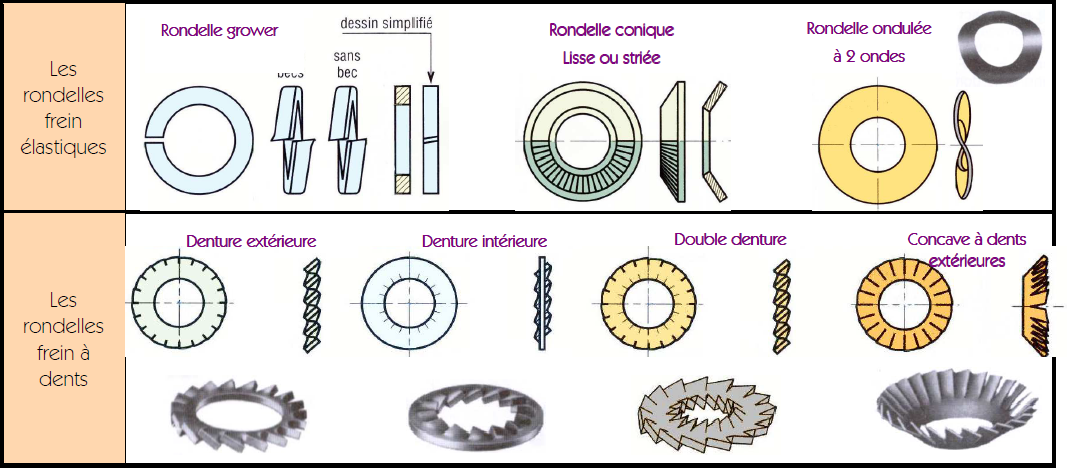
\includegraphics[width=.8\textwidth]{png/rondelles}
\end{center}

\section{Assurer la mise en position}

Classiquement les vis ne sont jamais utilisées pour faire de la mise en position. Cependant, pour les conceptions où peu d'efforts transitent, certaines vis permettent d'assurer cette fonction.

\section{Quelques exemples d'outils}

\begin{center}
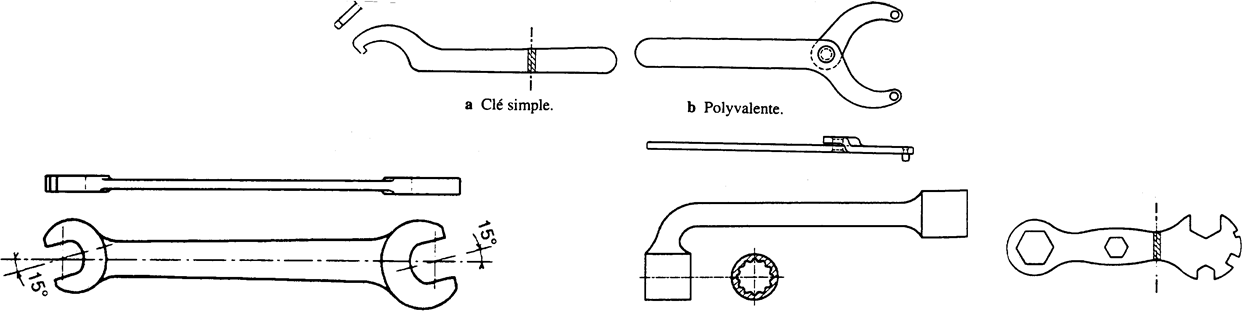
\includegraphics[width=.8\textwidth]{png/cles}
\end{center}



\begin{thebibliography}{2}
%\bibitem{ls}{\url{http://www.hellopro.fr/images/produit-2/2/4/9/motoreducteur-a-sortie-axiale-207942.jpg}}
%\bibitem{sew}{\url{http://www.cnr-cmao.ens-cachan.fr/fiches_dossiers/motoreducteur_sew_r17_DT.php?t=13}}
%\bibitem{poclain}{\url{http://www.cnr-cmao.ens-cachan.fr/}}
%\bibitem{poclain}{Fabrication de vis : \url{http://www.youtube.com/watch?v=7ORomNNCSUQ}}
%\bibitem{attachements}{http://www.gbmo.eu/attachement-pour-le-fraisage.html}
%\bibitem{attachements_2}{http://www.maritool.com/images/HSK50A-ER32-COLLET-CHUCK-1.jpg}
%\bibitem{mc}{Supports de cours de Maryline Carrez, Lycée Jules Haag, Besançon}
%\bibitem{rivets}{\url{http://www.linternaute.com/paris/magazine/photo/la-tour-eiffel-dans-tous-ses-etats/image/rivets-d-eiffel-441056.jpg}}

\bibitem{papier}{\url{http://membres.multimania.fr/solokoy/img/Joints\%20papier.jpg}}
\bibitem{torique}{\url{http://www.via-industry.com/rep_images/client/magicap/jointstoriques.jpg}}
\bibitem{culasse}{\url{http://www.vlvautoparts.com/vlvautoparts_images/produits/12.4726.jpg}}

\bibitem{mc}{Supports de cours de Maryline Carrez, Lycée Jules Haag, Besançon}
\bibitem{pf}{Supports de cours de Philippe Fichou, Lycée Vauban, Brest \url{http://philippe.fichou.pagesperso-orange.fr/documents/liaisoncomplete2003.pdf}}
\bibitem{pf}{Supports de cours de Jean-Pierre Pupier, Lycée Rouvière, Toulon}
\end{thebibliography}

\end{document}